%% ****** Start of file apsguide4-2.tex ****** %
%%
%%   This file is part of the APS files in the REVTeX 4.2 distribution.
%%   Version 4.2b of REVTeX, December 2018.
%%
%%   Copyright (c) 2019 The American Physical Society.
%%
%%   See the REVTeX 4.2 README file for restrictions and more information.
%%
\documentclass[twocolumn,secnumarabic,amssymb, nobibnotes, aps, prd]{revtex4-2}
\usepackage{graphicx}
%\usepackage{acrofont}%NOTE: Comment out this line for the release version!
\newcommand{\revtex}{REV\TeX\ }
\newcommand{\classoption}[1]{\texttt{#1}}
\newcommand{\macro}[1]{\texttt{\textbackslash#1}}
\newcommand{\m}[1]{\macro{#1}}
\newcommand{\env}[1]{\texttt{#1}}
\setlength{\textheight}{9.5in}

\begin{document}

\title{APS Author Guide for \revtex~4.2}%

\author{American Physical Society}%
\email[REVTeX Support: ]{revtex@aps.org}
\affiliation{1 Research Road, Ridge, NY 11961}
\date{December 2018}%
\maketitle
\tableofcontents

\section{Introduction}
This is a reference to \cite{DelaunayTriangulation1997}. And now a second reference \cite{gomppernelson2012}. Also, a third reference \cite{Helfrich1973}.


Articles published in American Physical Society journals are converted to 
an XML file during final journal production. Other formats such
as PDF are derived directly from the XML, which constitutes the version of record. 
Even before journal production, the APS editorial process can make use
of the information in a properly prepared manuscript. Information such
as title, authors, affiliations, etc., can be automatically
extracted and used to populate our manuscript database. References can
also be culled, cross-checked for accuracy, and used to create a
linked version for referees and editors. Moreover, time can be saved
as referrals can be made electronically rather than by conventional
mail. Thus, a well-prepared electronic manuscript can enhance the
entire peer review process from author to reader while making the
whole process less expensive. To this end, authors should follow the
guidelines in this document when preparing their submissions to \textit{Physical Review Letters},
 \textit{Reviews of Modern Physics},  \textit{Physical Review A-E, Physical Review X, Physical Review Applied. Physical Review Fluids, Physical Review Materials, Physical Review Accelerators and Beams,} and \textit{Physical Review Physics Education Research}.
 
Updated versions of this document will be made available at  \url{https://journals.aps.org/revtex/}. For more complete
descriptions of how to use the \revtex\ 4.2 macros, please see the
\textit{\revtex~4.2 Author's Guide} included with the \revtex~4.2
distribution. Questions about \revtex\ 4.2 and using it to submit to APS journals may be
emailed to \texttt{revtex@aps.org}.

\begin{figure}[htbp]
\begin{center}
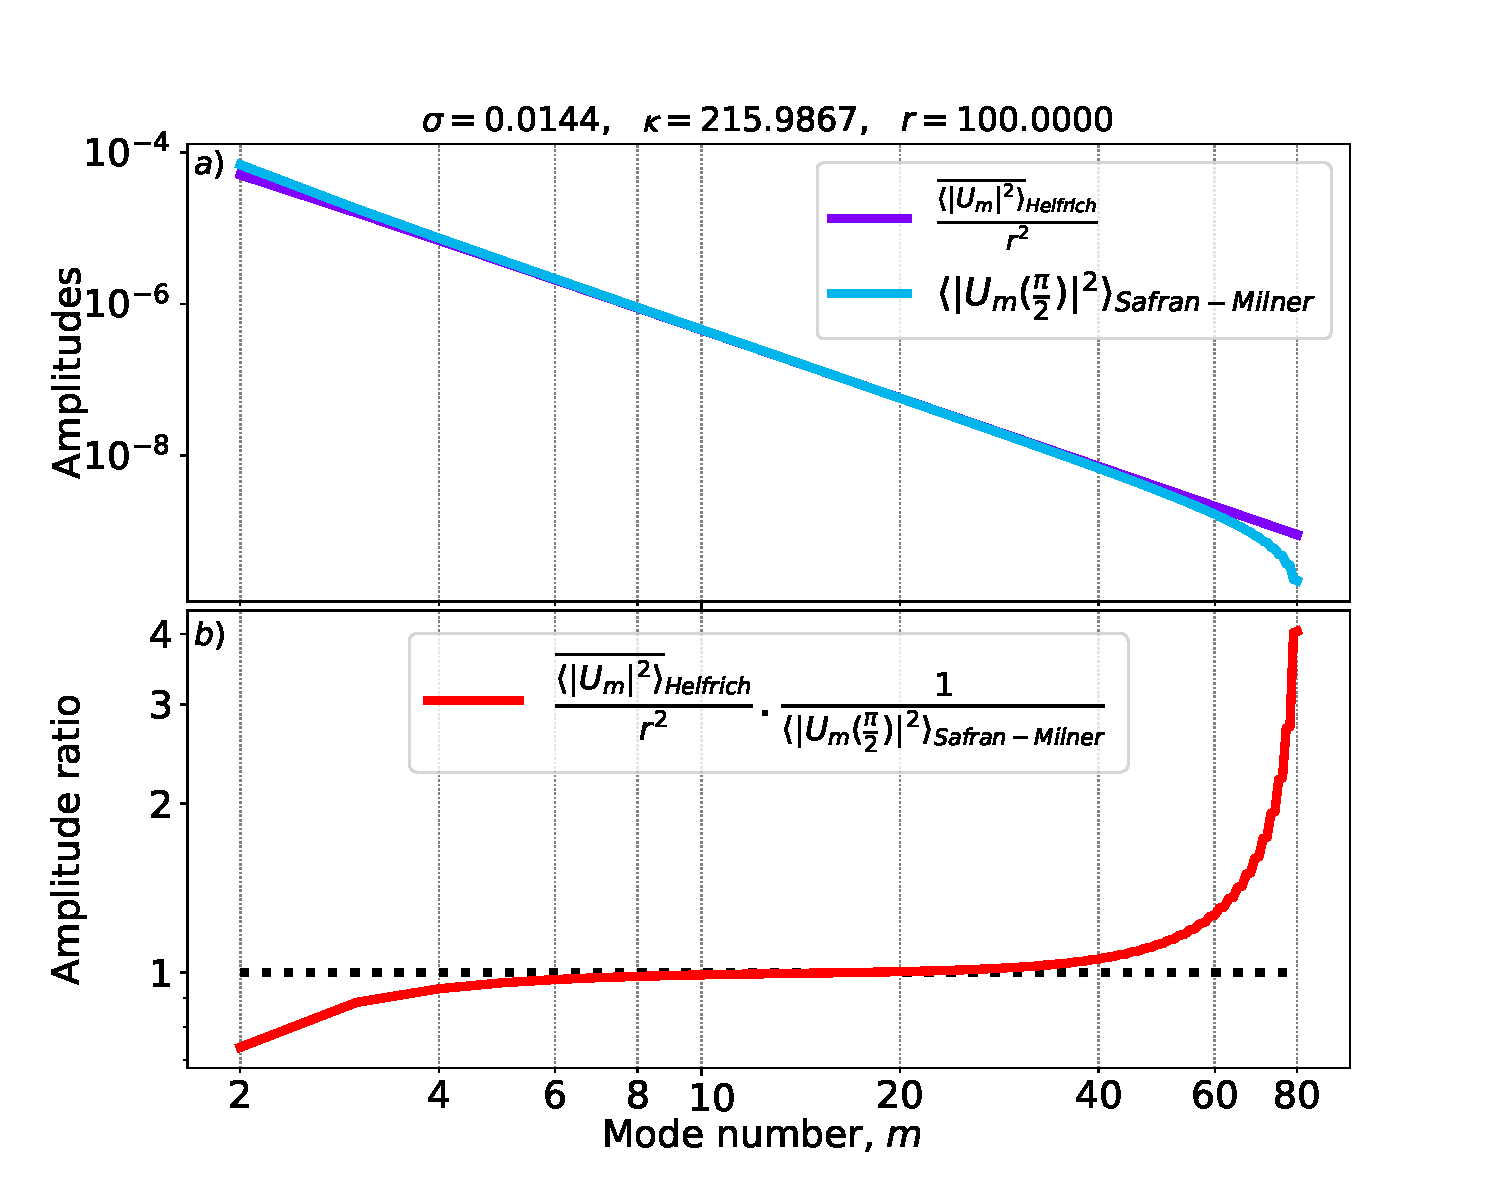
\includegraphics[width=8.5cm]{Fig1.pdf}
\caption{default}
\label{default}
\end{center}
\end{figure}





\section{Formatting}
\subsection{Preprint, reprint, and twocolumn options}
\revtex~4.2 offers a \classoption{reprint} class option to typeset a manuscript
in a format that is a close approximation to the actual journal's appearance. It should
be emphasized that this is only an \textit{approximation}; a manuscript may be substantially different
in length or appearance after it goes through our production process. This is mostly due to the choice
of fonts and the scaling of figures.

\revtex\ 4.2 is designed to
make it straightforward to switch between two-column and single-column
formatting just by changing the class option. Authors may submit with
either the \classoption{reprint} or the \classoption{twocolumn} class options.
The \classoption{preprint} primarily does three things: It increases
the font size to 12pt, increases the line spacing, and changes the
formatting to single column.

\subsection{Paper size}
Manuscripts should be submitted to APS formatted for letter size
paper. Papers are sent electronically to referees who may
want to print them out. Letter size formatting ensures that this will
be trouble free for all referees.

\section{Marking up front matter}
Perhaps the most important macros are those 
pertaining to the markup of the front matter (title, authors,
affiliations, abstract, etc.). Note that proper
use of the \revtex\ 4.2 macros means that explicit centering environments
in the front matter are not needed and should not be used.

\subsection{Title}
The title of the manuscript should be specified using the \m{title} macro. A
double backslash {\textbackslash\textbackslash} may be used to force a line break in a long
title.

\subsection{Authors, affiliations, and collaborations}
\label{sec:authors}
\revtex\ 4.2 makes it straightforward to input author names and link them up properly with affiliations. Authors should let \revtex\ 4.2 do the work of grouping authors and affiliations and, if using the superscript style, numbering affiliations. Please follow these guidelines:
\begin{itemize}
\item Use a single \m{author} macro for each author's name. \revtex\ 4.2 automatically puts in all commas and the word `and.'
\item Use the \m{surname} macro to explicitly indicate if an author's family name consists of more than one name or if the family name is not the author's last name.
\item The \m{email} macro may be used to specify an author's e-mail
address. The \m{thanks} macro must not be used for this. Only the
e-mail address itself may appear in the macro's required argument.
\item The \m{homepage} macro may be used to specify a URL associated
with an author. The \m{thanks} macro must not be used for this. Only the
URL may appear in the macro's required argument.
\item The \m{altaffiliation} macro may be used to specify an alternate
affiliation or temporary address for an author. The \m{thanks} macro
must not be used for this. Only the affiliation
may appear in the macro's required argument.
\item The \m{thanks} macro may be used only if one of the more
specific macros list above does not apply.
\item Use a single \m{affiliation} for each affiliation.
\item Superscripts linking authors to affiliations must be
accomplished using the \classoption{superscriptaddress} class option
rather than putting in explicit superscripts by hand.
\item A collaboration may be specified by using the \m{collaboration}
macro. The \m{author} macro must not be used for collaborations.
\end{itemize}
\subsection{Abstract}
The abstract must be specified using the \env{abstract}
environment. Note that in \revtex\ 4.2, the abstract must come before
the \m{maketitle} command. \revtex\ 4.2 now allows the the use of the \env{description}
environment within the abstract to provide \textit{structured abstracts}. For instance, \textit{Physical Review C} would like authors to provide abstracts with sections summarizing the paper's  \textbf{Background}, \textbf{Purpose}, \textbf{Method}, \textbf{Results}, and \textbf{Conclusions}. This can be accomplished in the following manner:
\begin{verbatim}
\begin{abstract}
\begin{description}
\item[Background] This part would describe the
context needed to understand what the paper
is about.
\item[Purpose] This part would state the purpose
of the present paper.
\item[Method] This part describe the methods
used in the paper.
\item[Results] This part would summarize the
results.
\item[Conclusions] This part would state the
conclusions of the paper.
\end{description}
\end{abstract}
\end{verbatim}

\section{References and footnotes}
Authors are strongly encouraged
to use Bib\TeX\ when preparing their bibliographies.  If Bib\TeX\ is used, current production processes
require that the \texttt{.bbl} file be included directly into the
manuscript's main \texttt{.tex} file. \revtex\ 4.2 comes with two Bib\TeX\ style files for formatting
references, one for the \textit{Physical Review} journals and one 
for \textit{Review of Modern Physics}. In 4.2, the Bib\TeX\ styles have been modified to display journal article titles in the bibliography.

The following apply whether
Bib\TeX\ is used or not.  
\begin{itemize}
\item Authors should use the \m{cite} and \m{bibitem} commands to create
bibliographies and to refer to items in the bibliography. ``By hand"
numbering of references should be avoided.
\item \revtex~4.2 provides new syntax for combining multiple citations into a single entry in the bibliography and for putting extra text before and after a reference. Please refer to \textit{\revtex~4.2 Author's Guide} included with the \revtex~4.2 distribution for full details.
\item Footnotes must be specified using the \m{footnote}
macro. \revtex\ 4.2 will place the footnotes in
the bibliography for the \textit{Physical Review}
journals. Please note that even if you don't use Bib\TeX, you may have to run Bib\TeX\ to get the footnotes to appear. Footnotes giving additional information about authors (such
as e-mail addresses) must not be specified using the \m{footnote}
macro (see Section~\ref{sec:authors}).
\item Avoid custom footnotes using \m{footnotemark} and \m{footnotetext} [except in the context of tables (see
Section~\ref{sec:tablenotes})].
\item References should be formatted and specified according to the
\textit{Physical Review Style Guide}. Note that using Bib\TeX\ automatically ensures this.
\item URLs should be specified using the \m{url} macro. Bib\TeX\ will automatically take
care of this if the \texttt{url} field is used.
\item E-print identifiers should be included using the \m{eprint} macro. Bib\TeX\ will automatically take care of this if the \texttt{eprint} field is used.
\end{itemize}

Please see the \revtex~4.2 Author's Guide for new features in \revtex~4.2's APS Bib\TeX\ styles, including support for citing data sets, journals that use DOIs in place of page numbers, and journals that use year and issue instead of volume to uniquely identify articles.

\section{Body of the paper}
\subsection{Sectioning and cross-referencing}
For sectioning a manuscript, the basic rule is to use the appropriate
sectioning commands (\m{section}, \m{subsection}, \m{subsubsection},
\textit{etc.}). Cross-referencing a section must be done by using the
proper \m{label} and \m{ref} commands. Cross-referencing by hand is
not allowed. \m{part}, \m{chapter}, and \m{subparagraph} should not be
used.

\subsection{Appendices}
Appendices should be specified using the \m{appendix} command which
specifies that all following sections create with the \m{section}
commands are appendices. If there is only one appendix, then the
\m{appendix*} command should be used instead.

\subsection{Acknowledgments}
Any acknowledgments should be included by using the
\env{acknowledgments} environment. Note that in \revtex~4.2, this is
an environment and not a command.

\subsection{Counters}
No counters may be created and the standard ones may not be
altered. If an exceptional label is needed for an equation, the \m{tag}
command (requires the \classoption{amsmath} class option) should be used. Please
note that the use of the \m{tag} command may conflict with the use of the \classoption{hyperref} package
due an incompatibility between \classoption{amsmath} and \classoption{hyperref}.

\subsection{Fonts}
It is preferable to avoid the older \TeX\ and \LaTeX\ 2.09 macros for
controlling fonts such as \m{rm}, \m{it}, \textit{etc.} Rather, it is
better to use the macros introduced in \LaTeXe.  If the older font
commands are used (they really should be avoided!), be sure to use
curly braces to properly limit the extent of the font
change. \verb+{\bf ...}+ is the correct method.
Commands for controlling text and math font changes are summarized in
Table~\ref{tab:fonts}.

\begin{table}
\caption{\label{tab:fonts}\LaTeXe\ and AMS-\LaTeX\ font summary.}
\begin{ruledtabular}
\begin{tabular}{lp{2in}}
\m{textit} & Italics. Replaces \m{it}\\
\m{textbf} & Bold face. Replaces \m{bf}\\
\m{textrm} & Roman. Replaces \m{rm}\\
\m{textsl} & Slanted. Replaces \m{sl}\\
\m{textsc} & Small caps. Replaces \m{sc}\\
\m{textsf} & Sans serif. Replaces \m{sf}\\
\m{texttt} & Typewriter. Replaces \m{tt}\\
\m{textmd} & Medium series\\
\m{textnormal} & Normal\\
\m{textup} & Upright\\
\m{mathbf} & Bold face\\
\m{mathcal} & Replaces \m{cal}\\
\m{mathit} & Italics\\
\m{mathnormal} & Replaces \m{mit}\\
\m{mathsf} & Sans serif\\
\m{mathtt} & Typewriter\\
\m{mathfrak} & Fraktur: Requires \classoption{amsfonts} or \classoption{amssymb} class option\\
\m{mathbb} & Bold blackboard: Requires \classoption{amsfonts} or \classoption{amssymb} class option\\
\m{bm} & Bold Greek and other math symbols: Requires
\verb+\usepackage{bm}+ and may require the \classoption{amsfonts} class
option
\end{tabular}
\end{ruledtabular}
\end{table}

Bold Greek letters and other bold math symbols should be accomplished
with the use of \texttt{bm.sty} which is distributed as a required
tool with the latest versions of \LaTeXe\ and should be loaded via
\verb+\usepackage{bm}+. This package introduces the \m{bm}
macro. Some bold characters may require using the
\classoption{amsfonts} class option.

New fonts may not be declared with \m{newfont}. Font attribute
commands for selecting a font family, shape, and series are all
disallowed; the standard \LaTeXe\ font selection macros list above
should be used instead.

Finally, the \m{symbol} macro is also not allowed.

\subsection{Environments}
\subsubsection{Lists}
The standard list environments \texttt{itemize}, \texttt{enumerate},
and \texttt{description} are allowed. The \m{item} macro with or without
the optional argument is also allowed. Customization of the list environments
(with macros such as \m{labelstyle}, \m{labelitemi}, \m{labelenumi},
\m{itemsep}, etc.) is allowed but may be ignored in production.
Generalized lists (\m{begin\{list\}}) and trivial lists
(\m{begin\{trivlist\}}) are not allowed.

\subsubsection{Other Environments}
Creating generalized new environments with \m{newenvironment} is not
allowed. Creating a new theorem environment with \m{newtheorem} is
allowed though.

The tabbing environment and the macros \m{=}, \m{$>$}, \m{`}, and
\m{'} are allowed but may be ignored in production. Conversion
programs used in production should recognize the escapes \m{a=},
\m{a'}, and \m{a`} for using the corresponding accents within a
tabbing environment though.

The \env{verbatim} environment is allowed.

\subsection{Boxes}
Most boxes and macros to manipulate them are not allowed. These
include \m{raisebox}, \m{parbox}, \m{minipage}, \m{rulebox},
\m{framebox}, \m{mbox}, \m{fbox}, \m{savebox}, \m{newsavebox},
\m{sbox}, \m{usebox}, and the environment \m{begin\{lrbox\}}. Rules
produced with \m{rule} are not allowed.

\subsubsection{Margin Notes}
Margin notes created with \m{marginpar} are not allowed, as are the
associated style parameters \m{marginparwidth}, \m{marginparsep}, and
\m{marginparpush}.


\section{Math Markup}
In general, all math markup and the standard math environments from
\LaTeXe\ are allowed. These include \m{begin\{math\}},
\m{begin\{displaymath\}}, \m{begin\{equation\}},
\m{begin\{eqnarray\}}, and \m{begin\{eqnarray*\}}. The shortcuts \$,
\$\$, \m{[}, and \m{]} are allowed. In addition, authors may use
almost all of the additional markup introduced by AMS-\LaTeX\ by using
the \classoption{amsmath} class option. The explicit exceptions are
\m{genfrac}, \m{boxed}, and \m{smash}. The markup contained in
\texttt{amsextra} and \texttt{amsthm} may not be used
though. Commutative diagrams created with the \texttt{amscd} package
are acceptable.

\section{Figures}
\subsection{Figure inclusions}
Figures should be included into a \revtex~4.2 manuscript by using the
standard \LaTeXe\ macros. \LaTeXe\ includes
several powerful packages for including the files in various
formats. The two main packages are \texttt{graphics} and
\texttt{graphicx}. Both offer a macro called
\m{includegraphics};
they mainly differ in how arguments for
controlling figure placement (\textit{e.g.}, scaling and rotation)
are passed to the \m{includegraphics}.

The \env{figure} environment should be used to add a caption to the
figure and to allow \LaTeX\ to number and place the figures where they
fit best.  If a figure needs to be referred to in the text,
rather than manually numbering the figures a \m{label} should be added
to the figure environment (best practice is to put the label within
the argument of the \m{caption} command) and the \m{ref} macro should be used to
reference this label. Figures that span the page should use the
\m{figure*} environment. The \env{picture} environment must not be
used directly (one can include an Encapsulated PostScript figure that
was produced using the \env{picture} environment of course).

\subsection{\label{sec:figplace}Figure placement}
Figures should be placed as close as possible to the point where they are first
referenced. There is no need to place all figures
separately at the end of the manuscript and it is preferred that
authors leave the figures in their natural locations. Authors may
also find useful the \revtex~4.2 \classoption{floatfix} class option
which adds emergency float placement processing to avoid ``stuck''
floats which would otherwise be deferred to the end of the job (and
can lead to the fatal \texttt{``Too many unprocessed floats''}
message).


\section{Tables}
\label{sec:tables}
The standard \LaTeXe\ table formatting environments are supported as is
the use of the \texttt{longtable} package. Tables may be reformatted
during production to meet APS style guidelines.
Here are some helpful hints for trying to get tables formatted correctly:
\begin{itemize}
\item Use the \texttt{longtable} package to get tables to break
across pages.
\item The macro \m{squeezetable} will reduce the font size of the
table. This macro must occur within a group outside the table
environment. The proper markup is:
\begin{verbatim}
\begingroup
\squeezetable
\begin{table}
...
\end{table}
\endgroup
\end{verbatim}
\item Try using the float placement option \texttt{H} which will
enable \LaTeX\ to break a float across pages. Long tables are more
attractively set with \env{longtable} however.
\begin{verbatim}
\begin{table}[H]
\begin{ruledtabular}
\begin{tabular}
...
\end{tabular}
\end{ruledtabular}
\end{table}
\end{verbatim}
\end{itemize}

\subsection{Doubled rules and table formatting}
\revtex\ 4.2 provides the \env{ruledtabular} environment which
automatically puts the scotch rules (double lines) around tables and
formats all enclosed \env{tabular} environments to the full width of
the tables and improves inter-column spacing. This environment should
be used whenever possible.

\subsection{Wide tables}
When typesetting using \classoption{twocolumn}, tables can either span
a single column or both columns. Using the '\verb+*+'-ed version of
the \env{table} or \env{longtable} environments produces wide tables
that span the columns.

Tables that are very wide and that may be better typeset in a
landscape orientation (rotated 90 degrees) should be enclosed in a
\env{turnpage} environment. This will place the rotated table on its own
page. Note that some dvi previewers may not be able to show the table
properly, but \texttt{dvips} and \texttt{pdflatex} work correctly.

\subsection{Table placement}
Tables should be placed as close as possible to the point where they
are first referenced. There is no need to place all tables separately
at the end of the manuscript and this is not desirable for APS
purposes. The class option \classoption{floatfix} may be helpful for
table placement as well as figure placement (see Section~\ref{sec:figplace}).

\subsection{Aligning columns on a decimal point}
The standard \LaTeXe\ macro package \classoption{dcolumn} should be
used to accomplish this.

\subsection{Tablenotes}
\label{sec:tablenotes}
Footnotes in tables (tablenotes) should use the \m{footnote}
macro. However, if more than one reference to the same footnote is
needed, authors may use \m{footnotetext} and \m{footnotemark}. This
will produce notes (labeled by lower-case roman letters) inserted
below the table rather than in the reference section or at the bottom
of the page.


\section{Author-defined macros}
Authors may define convenience macros to save keystrokes. This means
that the macros may not invoke \TeX\ macros such as \m{if} or other
context dependent commands. Also, \LaTeXe\ provides three macros for
declaring new commands: \m{providecommand}, \m{newcommand}, and
\m{renewcommand} (as well as their `\verb+*+'-ed versions). These
should be used. Authors may not use \TeX\relax's low-level commands
\m{def}, \m{edef}, and \m{gdef}.

\section{Summary}
To ensure the best use of \TeX\ manuscripts, authors need to follow
the guidelines specified here. Use of low-level formatting commands to
finely control horizontal and vertical spacing may be ignored during
production, or even worse, make it impossible to convert the
manuscript to XML. Authors should keep
things as simple as possible and correctly use the proper \revtex~4.2
or \LaTeXe\ macros. Any questions about usage may be directed to
\texttt{revtex@aps.org}.
\bibliography{paper2.bib
%/Users/ali/Documents/Dr\ Ejtehadi/PhD-Thesis/reference.bib
%../../../Dr\ Ejtehadi/PhD-Thesis/reference.bib
}
\end{document}

